% Source PDF page 365 (printed p. 351)
\section{参数化分布估计}
\subsection{最大似然估计}
考虑 $\R^m$ 上由向量 $x\in\R^n$ 索引的一族概率分布，其密度为 $p_x(\cdot)$。固定 $y\in\R^m$，将 $p_x(y)$ 看成 $x$ 的函数时，称其为\emph{似然函数}。使用它的对数更方便，这个对数称为\emph{对数似然函数}，记作 $l$：
\[
 l(x)=\log p_x(y).
\]
参数 $x$ 的取值往往有约束，可以表示关于 $x$ 的先验知识，也可以表示似然函数的定义域。这些约束可以显式给出，也可以包含在似然函数中：只要 $x$ 不满足先验信息约束，就对所有 $y$ 令 $p_x(y)=0$。因此，对违反先验信息约束的参数 $x$，可以将对数似然函数赋值为 $-\infty$。

现在，考虑根据从分布中观测到的一个样本 $y$ 估计参数 $x$。一种广泛使用的方法是\emph{最大似然}（ML）估计，将 $x$ 估计为
\[
 \widehat x_{\mathrm{ml}}=\argmax_xp_x(y)=\argmax_xl(x),
\]
即选择使观测值 $y$ 的似然函数或对数似然函数最大的参数值作为估计。如果存在关于 $x$ 的先验信息，例如 $x\in C\subseteq\R^n$，则可显式加入约束 $x\in C$，或者对 $x\notin C$ 重新定义 $p_x(y)=0$，从而隐式施加这一约束。

寻找参数向量 $x$ 的最大似然估计，可以写为
\begin{equation}
\begin{array}{ll}
\text{最大化}&l(x)=\log p_x(y)\\
\text{满足}&x\in C,
\end{array}\tag{7.1}
\end{equation}
其中 $x\in C$ 表示参数向量的先验信息或其他约束。在该优化问题中，向量 $x\in\R^n$，即概率密度中的参数，是优化变量；向量 $y\in\R^m$，即观测样本，是问题参数。

% Source PDF page 366 (printed p. 352)
如果对每个 $y$，对数似然函数 $l$ 都凹，而且集合 $C$ 能用线性等式和凸不等式约束描述，那么最大似然估计问题（7.1）就是凸优化问题。许多估计问题都属于这种情形，可以用凸优化计算ML估计。

\subsubsection*{具有独立同分布噪声的线性测量}
考虑线性测量模型
\[
 y_i=a_i^{\T}x+v_i,\qquad i=1,\ldots,m,
\]
其中 $x\in\R^n$ 是待估参数向量，$y_i\in\R$ 为测量或观测量，$v_i$ 是测量误差或噪声。假设 $v_i$ 独立同分布（IID），在 $\R$ 上的密度为 $p$，则似然函数为
\[
 p_x(y)=\prod_{i=1}^mp(y_i-a_i^{\T}x),
\]
从而对数似然函数为
\[
 l(x)=\log p_x(y)=\sum_{i=1}^m\log p(y_i-a_i^{\T}x).
\]
ML估计为下列问题的任意最优点：
\begin{equation}
 \text{最大化}\quad\sum_{i=1}^m\log p(y_i-a_i^{\T}x),\tag{7.2}
\end{equation}
变量为 $x$。如果密度 $p$ 对数凹，则该问题凸，并具有罚函数逼近问题的形式，罚函数为 $-\log p$，见第294页（6.2）。

\begin{origexample}{7.1}
\textbf{几种常见噪声密度的ML估计。}
\begin{itemize}
\item \emph{高斯噪声。}若 $v_i$ 服从零均值、方差为 $\sigma^2$ 的高斯分布，其密度为
\[
 p(z)=(2\pi\sigma^2)^{-1/2}e^{-z^2/(2\sigma^2)},
\]
对数似然函数为
\[
 l(x)=-(m/2)\log(2\pi\sigma^2)-\frac1{2\sigma^2}\norm{Ax-y}_2^2,
\]
其中 $A$ 的各行为 $a_1^{\T},\ldots,a_m^{\T}$。因此，$x$ 的ML估计为 $x_{\mathrm{ml}}=\argmin_x\norm{Ax-y}_2^2$，即最小二乘逼近问题的解。
\item \emph{Laplace噪声。}若 $v_i$ 服从Laplace分布，密度为 $p(z)=(1/2a)e^{-\abs z/a}$，其中 $a>0$，则ML估计为 $\widehat x=\argmin_x\norm{Ax-y}_1$，即 $\ell_1$ 范数逼近问题的解。
\item \emph{均匀噪声。}若 $v_i$ 在 $[-a,a]$ 上均匀分布，则在该区间有 $p(z)=1/(2a)$，任意满足 $\norm{Ax-y}_\infty\le a$ 的 $x$ 都是一个ML估计。
\end{itemize}
\end{origexample}

% Source PDF page 367 (printed p. 353)
\subsubsection*{罚函数逼近的ML解释}
反过来，任意罚函数逼近问题
\[
 \text{最小化}\quad\sum_{i=1}^m\phi(b_i-a_i^{\T}x)
\]
都可以解释为测量值为 $b$、噪声密度为
\[
 p(z)=\frac{e^{-\phi(z)}}{\int e^{-\phi(u)}\,\mathrm du}
\]
的最大似然估计问题。这个观察为罚函数逼近提供了统计解释。例如，假设罚函数 $\phi$ 在较大取值处增长极快，意味着对大的残差赋予很大的代价或惩罚。相应噪声密度 $p$ 的尾部会很小；ML估计器将尽可能避免产生大残差，因为这些残差对应极不可能发生的事件。

也可从最大似然估计的角度理解，为什么 $\ell_1$ 范数逼近对大误差稳健。$\ell_1$ 范数逼近对应Laplace噪声密度下的最大似然估计，$\ell_2$ 范数逼近对应高斯噪声密度下的最大似然估计。Laplace密度的尾部比高斯密度更大，也就是说，Laplace分布下出现很大 $v_i$ 的概率远高于高斯分布。因此，相应最大似然方法预期会遇到更多的大残差。

\subsubsection*{Poisson分布的计数问题}
许多问题中的随机变量 $y$ 取非负整数值，服从均值 $\mu>0$ 的Poisson分布：
\[
 \Prob(y=k)=\frac{e^{-\mu}\mu^k}{k!}.
\]
$y$ 常常表示某段时间内Poisson过程的事件次数，例如光子到达次数、交通事故数等。

在一个简单的统计模型中，将均值 $\mu$ 建模为向量 $u\in\R^n$ 的仿射函数：
\[
 \mu=a^{\T}u+b.
\]
$u$ 称为\emph{解释变量}向量，$a\in\R^n$ 和 $b\in\R$ 称为\emph{模型参数}。例如，若 $y$ 是某地区某时段的交通事故数，$u_1$ 可以是该时段经过该地区的总交通流量，$u_2$ 可以是该时段该地区的降雨量，等等。

给定若干观测对 $(u_i,y_i)$，$i=1,\ldots,m$，其中 $y_i$ 是解释变量取 $u_i\in\R^n$ 时观测到的 $y$。任务是由这些数据找到模型参数 $a\in\R^n$、$b\in\R$ 的最大似然估计。

% Source PDF page 368 (printed p. 354)
似然函数为
\[
 \prod_{i=1}^m\frac{(a^{\T}u_i+b)^{y_i}\exp(-(a^{\T}u_i+b))}{y_i!},
\]
所以对数似然函数为
\[
 l(a,b)=\sum_{i=1}^m\bigl(y_i\log(a^{\T}u_i+b)-(a^{\T}u_i+b)-\log(y_i!)\bigr).
\]
通过求解凸优化问题
\[
 \text{最大化}\quad\sum_{i=1}^m\bigl(y_i\log(a^{\T}u_i+b)-(a^{\T}u_i+b)\bigr),
\]
便可找到 $a$、$b$ 的ML估计，变量为 $a,b$。

\subsubsection*{Logistic回归}
考虑随机变量 $y\in\{0,1\}$，满足
\[
 \Prob(y=1)=p,\qquad\Prob(y=0)=1-p,
\]
其中 $p\in[0,1]$，假设它依赖解释变量向量 $u\in\R^n$。例如，$y=1$ 可以表示某人患某种疾病，患病概率为 $p$。将 $p$ 建模为解释变量 $u$ 的函数，这些解释变量可以是体重、年龄、身高、血压及其他医学相关变量。

\emph{Logistic模型}的形式为
\begin{equation}
 p=\frac{\exp(a^{\T}u+b)}{1+\exp(a^{\T}u+b)},\tag{7.3}
\end{equation}
其中模型参数 $a\in\R^n$、$b\in\R$ 确定概率 $p$ 如何随解释变量 $u$ 变化。

现给定解释变量 $u_1,\ldots,u_m\in\R^n$ 及相应结果 $y_1,\ldots,y_m\in\{0,1\}$ 组成的数据，任务是找到模型参数 $a\in\R^n$、$b\in\R$ 的最大似然估计。求 $a,b$ 的ML估计有时称为\emph{Logistic回归}。

可重排数据，使 $u_1,\ldots,u_q$ 对应 $y=1$，$u_{q+1},\ldots,u_m$ 对应 $y=0$。似然函数为
\[
 \prod_{i=1}^q p_i\prod_{i=q+1}^m(1-p_i),
\]
其中 $p_i$ 由解释变量取 $u_i$ 的Logistic模型给出。对数似然函数为
\[
 l(a,b)=\sum_{i=1}^q\log p_i+\sum_{i=q+1}^m\log(1-p_i).
\]

% Source PDF page 369 (printed p. 355)
\begin{figure}[htbp]\centering
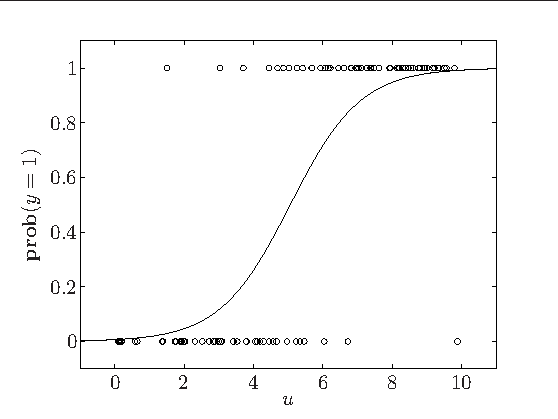
\includegraphics[width=.70\textwidth]{figures/ch07-figure-1.pdf}
\caption*{图7.1\quad Logistic回归。圆圈表示50个点 $(u_i,y_i)$，其中 $u_i\in\R$ 是解释变量，$y_i\in\{0,1\}$ 是结果。数据表明，当 $u$ 小于约5时，结果更可能为 $y=0$；当 $u$ 大于约5时，更可能为 $y=1$。此外，当 $u$ 小于约2时，$y=0$ 的可能性很高；当 $u$ 大于约8时，$y=1$ 的可能性很高。实线为最大似然参数 $a,b$ 对应的 $\Prob(y=1)=\exp(au+b)/(1+\exp(au+b))$。这个最大似然模型与我们对数据的非正式观察一致。}
\end{figure}
继续化简得
\[
\begin{aligned}
 l(a,b)&=\sum_{i=1}^q\log\frac{\exp(a^{\T}u_i+b)}{1+\exp(a^{\T}u_i+b)}
       +\sum_{i=q+1}^m\log\frac1{1+\exp(a^{\T}u_i+b)}\\
 &=\sum_{i=1}^q(a^{\T}u_i+b)-\sum_{i=1}^m\log(1+\exp(a^{\T}u_i+b)).
\end{aligned}
\]
由于 $l$ 关于 $a,b$ 凹，Logistic回归可作为凸优化问题求解。图7.1给出了 $u\in\R$ 时的一个例子。

\subsubsection*{高斯变量的协方差估计}
设 $y\in\R^n$ 是零均值高斯随机变量，协方差矩阵为 $R=\E yy^{\T}$，则其密度为
\[
 p_R(y)=(2\pi)^{-n/2}\det(R)^{-1/2}\exp(-y^{\T}R^{-1}y/2),
\]
其中 $R\in\mathbf S_{++}^n$。我们希望根据从分布中抽取的 $N$ 个独立样本 $y_1,\ldots,y_N\in\R^n$，并利用关于 $R$ 的先验知识，估计协方差矩阵 $R$。

对数似然函数为
\[
 l(R)=\log p_R(y_1,\ldots,y_N).
\]

% Source PDF page 370 (printed p. 356)
展开得到
\[
\begin{aligned}
 l(R)&=-(Nn/2)\log(2\pi)-(N/2)\log\det R
       -(1/2)\sum_{k=1}^N y_k^{\T}R^{-1}y_k\\
 &=-(Nn/2)\log(2\pi)-(N/2)\log\det R
       -(N/2)\tr(R^{-1}Y),
\end{aligned}
\]
其中
\[
 Y=\frac1N\sum_{k=1}^N y_ky_k^{\T}
\]
是 $y_1,\ldots,y_N$ 的样本协方差。该对数似然函数关于 $R$ 不凹，尽管它在定义域 $\mathbf S_{++}^n$ 的某个子集上凹，见习题7.4；但变量变换可得到凹的对数似然函数。用 $S=R^{-1}$ 表示协方差的逆，称其为\emph{信息矩阵}。以 $S$ 代替 $R$ 作为新参数，对数似然函数成为
\[
 l(S)=-(Nn/2)\log(2\pi)+(N/2)\log\det S-(N/2)\tr(SY),
\]
它关于 $S$ 凹。

因此，求解
\begin{equation}
\begin{array}{ll}
\text{最大化}&\log\det S-\tr(SY)\\
\text{满足}&S\in\mathcal S
\end{array}\tag{7.4}
\end{equation}
即可得到 $S$，进而得到 $R$ 的ML估计，其中集合 $\mathcal S$ 表示对 $S=R^{-1}$ 的先验知识，此外还有隐式约束 $S\in\mathbf S_{++}^n$。目标函数凹，因此当 $\mathcal S$ 能由线性等式与凸不等式约束描述时，该问题凸。

先考察除 $R\succ0$ 外，对 $R$，从而对 $S$，不作其他先验假设的情形。这时（7.4）可解析求解。目标的梯度为 $S^{-1}-Y$，所以当 $Y\in\mathbf S_{++}^n$ 时，最优 $S$ 满足 $S^{-1}=Y$。如果 $Y\notin\mathbf S_{++}^n$，对数似然函数上无界。因此，不对 $R$ 作先验假设时，协方差的最大似然估计就是样本协方差：$\widehat R_{\mathrm{ml}}=Y$。

再考虑可表示为信息矩阵 $S$ 的凸约束的一些 $R$ 约束。$R$ 的矩阵下界与上界
\[
 L\preceq R\preceq U,
\]
其中 $L,U$ 对称正定，可以写成
\[
 U^{-1}\preceq R^{-1}\preceq L^{-1}.
\]
关于 $R$ 的条件数约束
\[
 \lambda_{\max}(R)\le\kappa_{\max}\lambda_{\min}(R)
\]
可写为
\[
 \lambda_{\max}(S)\le\kappa_{\max}\lambda_{\min}(S).
\]

% Source PDF page 371 (printed p. 357)
这等价于存在 $u>0$，使 $uI\preceq S\preceq\kappa_{\max}uI$。因此，带 $R$ 条件数约束的ML估计，可以通过求解凸问题
\begin{equation}
\begin{array}{ll}
\text{最大化}&\log\det S-\tr(SY)\\
\text{满足}&uI\preceq S\preceq\kappa_{\max}uI
\end{array}\tag{7.5}
\end{equation}
得到，变量为 $S\in\mathbf S^n$ 和 $u\in\R$。

另一个例子是，对底层随机向量 $y$ 的若干线性函数的方差给出上界：
\[
 \E(c_i^{\T}y)^2\le\alpha_i,\qquad i=1,\ldots,K.
\]
这些先验假设可以表示为
\[
 \E(c_i^{\T}y)^2=c_i^{\T}Rc_i=c_i^{\T}S^{-1}c_i\le\alpha_i,
 \qquad i=1,\ldots,K.
\]
由于 $S\succ0$ 时 $c_i^{\T}S^{-1}c_i$ 是 $S$ 的凸函数，而此处正满足这一条件，因此可以在ML问题中施加这些界。

\subsection{最大后验概率估计}
\emph{最大后验概率}（MAP）估计可看作最大似然估计的Bayes版本，它在底层参数 $x$ 上给定先验概率密度。假设 $x$，即待估向量，以及 $y$，即观测量，都是随机变量，联合密度为 $p(x,y)$。这与前述统计估计设定不同，在那里 $x$ 是参数，而非随机变量。

$x$ 的先验密度为
\[
 p_x(x)=\int p(x,y)\,\mathrm dy.
\]
这个密度表示观测向量 $y$ 之前，对 $x$ 可能取值的先验信息。类似地，$y$ 的先验密度为
\[
 p_y(y)=\int p(x,y)\,\mathrm dx,
\]
它表示对测量或观测向量 $y$ 的先验信息。

给定 $x$ 时 $y$ 的条件密度为
\[
 p_{y\mid x}(x,y)=\frac{p(x,y)}{p_x(x)}.
\]
在MAP估计中，$p_{y\mid x}$ 起到最大似然设定下参数相关密度 $p_x$ 的作用。给定 $y$ 时 $x$ 的条件密度为
\[
 p_{x\mid y}(x,y)=\frac{p(x,y)}{p_y(y)}
 =\frac{p_{y\mid x}(x,y)p_x(x)}{p_y(y)}.
\]

% Source PDF page 372 (printed p. 358)
将观测到的 $y$ 代入 $p_{x\mid y}$，得到 $x$ 的\emph{后验密度}，它表示观测之后关于 $x$ 的知识。

MAP方法根据观测 $y$ 对 $x$ 作如下估计：
\[
\begin{aligned}
 \widehat x_{\mathrm{map}}&=\argmax_xp_{x\mid y}(x,y)\\
 &=\argmax_xp_{y\mid x}(x,y)p_x(x)\\
 &=\argmax_xp(x,y).
\end{aligned}
\]
换言之，取在给定观测 $y$ 时，使 $x$ 的条件密度最大的值作为估计。这个估计与最大似然估计的唯一区别，是这里多出了第二项 $p_x(x)$，它可解释为对 $x$ 先验知识的考虑。若 $x$ 的先验密度在集合 $C$ 上均匀，则寻找MAP估计，就等价于在 $x\in C$ 约束下最大化似然函数，即ML估计问题（7.1）。

取对数，可将MAP估计写成
\begin{equation}
 \widehat x_{\mathrm{map}}
 =\argmax_x\bigl(\log p_{y\mid x}(x,y)+\log p_x(x)\bigr).\tag{7.6}
\end{equation}
第一项与对数似然函数基本相同；第二项按先验密度惩罚不太可能的 $x$，即 $p_x(x)$ 很小的 $x$。

暂且撇开两种设定在思想上的差异，通过（7.6）寻找MAP估计与通过（7.1）寻找ML估计，唯一的不同，是优化问题中多了一个与 $x$ 先验密度相关的项。因此，对任何具有凹对数似然函数的最大似然估计问题，都可以加入 $x$ 的对数凹先验密度，所得MAP估计问题仍凸。

\subsubsection*{具有独立同分布噪声的线性测量}
设 $x\in\R^n$ 与 $y\in\R^m$ 的关系为
\[
 y_i=a_i^{\T}x+v_i,\qquad i=1,\ldots,m,
\]
其中 $v_i$ 独立同分布，在 $\R$ 上的密度为 $p_v$，$x$ 在 $\R^n$ 上的先验密度为 $p_x$。于是 $x,y$ 的联合密度为
\[
 p(x,y)=p_x(x)\prod_{i=1}^mp_v(y_i-a_i^{\T}x),
\]
MAP估计可由求解优化问题
\begin{equation}
 \text{最大化}\quad\log p_x(x)+\sum_{i=1}^m\log p_v(y_i-a_i^{\T}x)\tag{7.7}
\end{equation}
得到。若 $p_x$ 与 $p_v$ 对数凹，这个问题凸。MAP问题（7.7）与对应ML问题（7.2）的唯一区别，是额外的 $\log p_x(x)$ 项。

% Source PDF page 373 (printed p. 359)
例如，如果 $v_i$ 在 $[-a,a]$ 上均匀分布，而 $x$ 的先验分布为均值 $\bar x$、协方差 $\Sigma$ 的高斯分布，那么求解二次规划
\[
\begin{array}{ll}
\text{最小化}&(x-\bar x)^{\T}\Sigma^{-1}(x-\bar x)\\
\text{满足}&\norm{Ax-y}_\infty\le a
\end{array}
\]
即可得到MAP估计，变量为 $x$。

\subsubsection*{精确线性测量的MAP估计}
设 $x\in\R^n$ 为待估参数向量，先验密度为 $p_x$。我们获得 $m$ 个精确，即无噪声、确定性的线性测量 $y=Ax$。换言之，给定 $x$ 时 $y$ 的条件分布，是集中在 $Ax$ 处、质量为一的点质量。MAP估计可由下列问题得到：
\[
\begin{array}{ll}
\text{最大化}&\log p_x(x)\\
\text{满足}&Ax=y.
\end{array}
\]
若 $p_x$ 对数凹，该问题凸。

如果在先验分布下，各参数 $x_i$ 独立同分布，在 $\R$ 上具有密度 $p$，则MAP估计问题为
\[
\begin{array}{ll}
\text{最大化}&\sum_{i=1}^n\log p(x_i)\\
\text{满足}&Ax=y,
\end{array}
\]
这是罚函数为 $\phi(u)=-\log p(u)$ 的最小罚问题，见第304页（6.6）。

反过来，任意最小罚问题
\[
\begin{array}{ll}
\text{最小化}&\phi(x_1)+\cdots+\phi(x_n)\\
\text{满足}&Ax=b
\end{array}
\]
均可解释为MAP估计问题，包含 $m$ 个精确线性测量 $Ax=b$，且 $x_i$ 独立同分布，密度为
\[
 p(z)=\frac{e^{-\phi(z)}}{\int e^{-\phi(u)}\,\mathrm du}.
\]

\section{非参数分布估计}
考虑取值于有限集合 $\{\alpha_1,\ldots,\alpha_n\}\subseteq\R$ 的随机变量 $X$。为简单起见，设其取值属于 $\R$；若取值属于 $\R^k$ 等空间，也可应用相同思想。$X$ 的分布由 $p\in\R^n$ 刻画，其中 $\Prob(X=\alpha_k)=p_k$。显然，$p$ 满足 $p\succeq0$、$\one^{\T}p=1$。反过来，如果 $p\in\R^n$ 满足这两个条件，就可通过 $\Prob(X=\alpha_k)=p_k$ 定义随机变量 $X$ 的概率分布。因此，概率单纯形
\[
 \{p\in\R^n\mid p\succeq0,\ \one^{\T}p=1\}
\]
与所有取值于 $\{\alpha_1,\ldots,\alpha_n\}$ 的随机变量 $X$ 的可能分布一一对应。

% Source PDF page 374 (printed p. 360)
本节讨论如何结合先验信息，以及可能获得的观测与测量，估计分布 $p$。

\subsubsection*{先验信息}
关于 $p$ 的许多先验信息，都能表示为线性等式或不等式约束。对任意函数 $f:\R\to\R$，
\[
 \E f(X)=\sum_{i=1}^np_if(\alpha_i)
\]
是 $p$ 的线性函数。特别地，若 $C\subseteq\R$，则 $\Prob(X\in C)$ 是 $p$ 的线性函数：
\[
 \Prob(X\in C)=c^{\T}p,\qquad
 c_i=\begin{cases}1&\alpha_i\in C,\\0&\alpha_i\notin C.\end{cases}
\]
因此，已知某些函数的期望值，例如矩，或者已知某些集合的概率，都能作为 $p\in\R^n$ 的线性等式约束加入。期望值或概率上的不等式，则能表示为 $p\in\R^n$ 的线性不等式。

例如，设已知 $X$ 的均值 $\E X=\alpha$、二阶矩 $\E X^2=\beta$，且 $\Prob(X\ge0)\le0.3$。这些先验信息可表示为
\[
 \E X=\sum_{i=1}^n\alpha_ip_i=\alpha,\qquad
 \E X^2=\sum_{i=1}^n\alpha_i^2p_i=\beta,\qquad
 \sum_{\alpha_i\ge0}p_i\le0.3,
\]
即关于 $p$ 的两个线性等式和一个线性不等式。

也可以加入涉及 $p$ 的非线性函数的先验约束。例如，$X$ 的方差为
\[
 \operatorname{var}(X)=\E X^2-(\E X)^2
 =\sum_{i=1}^n\alpha_i^2p_i-\left(\sum_{i=1}^n\alpha_ip_i\right)^2.
\]
第一项关于 $p$ 线性，第二项是 $p$ 的凹二次函数，所以 $X$ 的方差关于 $p$ 凹。因此，$X$ 方差的下界能表示为 $p$ 的凸二次不等式。

再例如，设 $A,B$ 为 $\R$ 的子集，考虑给定 $B$ 时 $A$ 的条件概率：
\[
 \Prob(X\in A\mid X\in B)=\frac{\Prob(X\in A\cap B)}{\Prob(X\in B)}.
\]
它是 $p\in\R^n$ 的线性分式函数，可以写为
\[
 \Prob(X\in A\mid X\in B)=c^{\T}p/d^{\T}p,
\]
其中
\[
 c_i=\begin{cases}1&\alpha_i\in A\cap B,\\0&\alpha_i\notin A\cap B,\end{cases}
 \qquad
 d_i=\begin{cases}1&\alpha_i\in B,\\0&\alpha_i\notin B.\end{cases}
\]
